\documentclass[a4paper]{article}
\usepackage[a4paper, total={6in, 9in}]{geometry}
\usepackage{graphicx}
%\setlength{\parindent}{0cm}
\usepackage{amsmath}
\usepackage{amssymb}
\usepackage{graphicx}
\usepackage{hyperref}
\usepackage{enumitem} 
\usepackage{hyperref}
\usepackage{graphicx}
\usepackage[parfill]{parskip}
\usepackage{lingmacros}
\usepackage{tree-dvips}
\usepackage{pythonhighlight}
\usepackage{graphicx}
\usepackage{caption}
\usepackage{subcaption}
\usepackage[export]{adjustbox}
\graphicspath{ {/home/user/Desktop/Cover Page} }
\begin{document}


% TITLE PAGE

\begin{titlepage}

\raggedleft

\includegraphics[scale=0.4]{Logo.png}\\

\vspace{3cm}
\begin{center}
\newcommand{\HRule}{\rule{\linewidth}{0.5mm}}
\textsc{\Large MATH3001: Project in Mathematics}\\[2.0mm]
\textsc{\Large School of Mathematics}\\[2.0mm]
\vspace{0.5cm}

	\HRule\\[0.4cm]

	{\huge\bfseries Using Random Numbers to Solve Problems in Maths and Physics}\\[0.4cm] 

	\HRule\\[1.5cm]

		\begin{minipage}{0.4\textwidth}
		\begin{flushleft}
			\large
			\textit{Author:}\\
			\text{Eleanor Sleightholm} \\
			\text{(201214895)}
		\end{flushleft}
	\end{minipage}
	~
	\begin{minipage}{0.4\textwidth}
		\begin{flushright}
			\large
			\textit{Supervisors:}\\
			\text{Dr Oliver Harlen} \\
			\text{Dr Mike Evans}
		\end{flushright}
	\end{minipage}
\mbox{}
\vfill
\text{December 11, 2020}

\end{center}
\end{titlepage}

% TABLE OF CONTENTS

\tableofcontents

% STARTING THE REPORT
\newpage
%\section{Interactions and Phase Transitions}
\parskip = \baselineskip
\section{General Introduction}


Monte Carlo (MC) methods are computational methods that solve various mathematical and physical problems to a particular accuracy using random numbers. The basic concept behind Monte Carlo methods is to use random sampling (also known as Monte Carlo sampling) to obtain numerical results.

Monte Carlo methods are widely used in the field of mathematics and physics and give rise to a number of groundbreaking discoveries in physics, game theory and finance. Although the Monte Carlo approach can be used in a whole range of different areas, the underlying fundamental aspect, random number generation to solve deterministic problems, remains paramount throughout. 

Monte Carlo sampling improves with accuracy in higher dimensions, specifically in terms of integration \cite{1}. One particular use of Monte Carlo methods is modelling the behaviour of atoms and molecules within a material. One of the fundamental pillars of physics, statistical mechanics, explores the collective behaviour of such molecules. Monte Carlo methods have been developed to understand and solve problems encountered by modelling these molecules in physical materials \cite{2}. Specifically, the “Metropolis Monte Carlo” method that will be incorporated with the Ising model and explored in Section 3.

This report will focus on the behaviour and study of atoms within a material and exhibit how Monte Carlo methods can be used to describe and visually represent physical phenomenon.

\section{Molecules in Materials - Boltzmann Distribution}

In statistical mechanics, observing the interaction between a large number of objects is key to understanding the behaviour of materials. Specifically, we can consider a given material made up of a vast amount of particles. This is known as a $system$ of particles. 

In a classical system of point particles, a microstate defines the position and momentum of every particle. For a single particle in one dimension, the microstates are the different positions of the particle. Equally, if the system is a group of particles then microstates correspond to the different arrangements of those particles \cite{2}.

The Boltzmann distribution \cite{3} is a key result from statistical mechanics and states that the probability of finding a physical system in a given microstate is, 
 \begin{align} 
p\textsubscript{i} = A\exp \Big( - \frac{E\textsubscript{i}}{k\textsubscript{B} T}\Big)
\end{align}
where ${k\textsubscript{B}}$ is the Boltzmann constant ($1.38$ $\times$ $10^{-23}JK^{-1}$ in standard units), $T$ is the absolute temperature and $E\textsubscript{i}$ is the energy of state $i$. The product $k_{B}T$ is the typical thermal energy associated with a degree of freedom. The normalisation constant, $A$, ensures that the total probability over all states, $i$, equals unity \cite{2}. That is, 
\begin{align*}
A^{-1} = \sum_{i}  \,\exp \Big( - \frac{E\textsubscript{i}}{k\textsubscript{B} T}\Big) 
\end{align*}
From the Boltzmann distribution, (1), we see immediately that states with low energies are more probable than states with high energies; as $E_{i} \rightarrow 0 $, $p_{i} \rightarrow 1$ and as $E_{i} \rightarrow \infty $, $p_{i} \rightarrow 0$. The Boltzmann distribution has many applications; specifically the Monte Carlo Metropolis algorithm which will be explored in further detail in Section 3.1.

\section{The Ising Model}
\parskip = \baselineskip
The Ising model \cite{4}, named after Ernst Ising, is a mathematical model of ferromagnetism in statistical mechanics. Ferromagnetism arises when a collection of atomic spins align such that their associated magnetic moments all point in the same direction, yielding a net magnetic moment. The Ising model is the simplest theoretical description of ferromagnetism. This model was invented by Wilhelm Lenz in 1920 and subsequently named after Ernst Ising who chose the model as a subject of his doctoral dissertation in 1925.
\parskip = \baselineskip

The Ising model works by representing each atom by an arrow that can point either up or down. This arrow
is also known as a “spin” and corresponds to the direction of the atom’s own magnetic moment. The model considers a lattice of size $N$ with spins at each lattice site that can
take only two values, ±$1$ (up or down respectively). We use the variable $\sigma_{i}$ to denote the
direction of the ith spin, with $\sigma_{i}$ = $+1$ representing up and  $\sigma_{i}$ = $-1$ representing down.
This lattice can be visually represented like in Figure 1(a) where blue arrows represent up spins ($+1$) and
red arrows represent down spins ($-1$).

\begin{figure}[h]
\centering
\begin{subfigure}{0.3\textwidth}
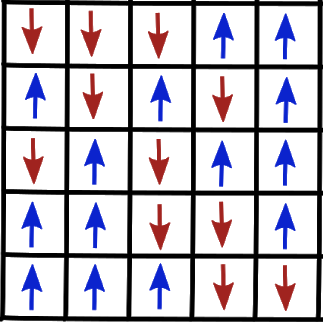
\includegraphics[width=1\linewidth]{lattice.png} 
\caption{A Lattice of Size 5}
\label{fig:subim1}
\end{subfigure}
\hspace{1cm}
\begin{subfigure}{0.2\textwidth}
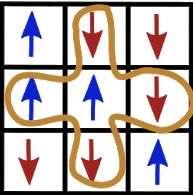
\includegraphics[width=1.1\linewidth]{nearestneighbours.png}
\vspace{0.6cm}
\caption{$<i, j>$}
\label{fig:subim2}
\end{subfigure}
\caption{Lattice Properties}
\label{fig:image2}
\end{figure}

Thus, if $N$ atoms are arranged on a lattice, like in Figure 1(a), then a state of the system can be represented by an array of $N$ values, each equal to ±$1$.
The total energy of the system is written:
\begin{equation}
E = -J\sum_{<i,j>} \sigma_{i}\sigma_{j} \, - h\sum_{i} \sigma_{i} \,
\end{equation}
where $<i,j>$ denotes that the summation is over the values of $i$ and $j$ that correspond to nearest neighbour spins; pairs of spins that are positioned next to each other on the lattice. This can be seen in Figure 1(b). Two neighbouring up spins or two neighbouring down spins have $\sigma_{i}\sigma_{j} = 1$ and two spins anti-aligned have $\sigma_{i}\sigma_{j}= -1$ \cite{2}. $J$ and $h$ are parameters of the model where $J$ refers to the exchange energy and $h$ refers to a positive magnetic field.

Using this equation, we are able to understand physical aspects of the Ising model. We notice that the first summation shows that the overall energy is lowered when neighbouring spins are aligned. Subsequently, the overall energy is heightened when neighbouring spins are anti-aligned. From this we can deduce that the Boltzmann distribution (1) gives preference to parallel alignment of neighbours. Similarly, the second summation will have lowest energy when spins in the lattice are pointing up ($\sigma_{i} = 1$). Thus, for the energy of the system to be at its lowest, all spins must be pointing upwards. 

\subsection{The Metropolis Algorithm for the Ising Model}

The Monte Carlo Metropolis algorithm \cite{5} can be used to transition a disordered (or anti-ferromagnetic) lattice of spins to an ordered (or ferromagnetic) lattice of spins.

As mentioned in Section 2, the Boltzmann distribution is used as an application to the Monte Carlo Metropolis Algorithm. The Metropolis algorithm was constructed to allow samples of microstates of a system to be taken with statistical weight in proportion to the Boltzmann distribution (1). 

Unlike Monte Carlo sampling methods, the Metropolis algorithm is a Markov Chain Monte Carlo (MCMC) method \cite{6} where it takes samples such that the next sample is dependent on an existing sample, called a Markov Chain. This method allows the Metropolis algorithm to narrow in on the quantity that is being approximated from the distribution, even with vast numbers of random variables. 

%The algorithm provided a break through in mathematics and statistical mechanics as it can be used to sample points from a probability distribution that would otherwise be difficult.

Adopting the Monte Carlo Metropolis algorithm to the Ising model \cite{7} allows a random array of spins to reach equilibrium magnetisation by iteration. The algorithm takes a random walk through the configuration space, visiting the more frequently-occurring spin configurations more often. The main steps for the Metropolis algorithm for the Ising model \cite{7} are as follows, 

\begin{description}[font=$\bullet$~\normalfont\scshape]
\item [Step 1] Start in an initial configuration of $N$ spins.
\item [Step 2] Choose a random lattice site and flip the spin, $\sigma_{i}$ located there.
\item [Step 3] Calculate the change in energy $\triangle{E_{i}}$. (This can be calculated using (2)).
\item [Step 4 (i)] If $\triangle{E_{i,j}} < 0$, accept the move.
\item [Step 4 (ii)] If not, then accept the move with probability, $\exp \Big( - \frac{\triangle{E_{i}}\textsubscript{i}}{k\textsubscript{B} T}\Big)$.
\item [Step 5] Repeat Steps 2 to 4 until the system reaches a equilibrium.
\end{description}

The Metropolis algorithm can be used to generate a random set of configurations of a system, drawn from the Boltzmann distribution. Thus, the algorithm can be used to model the behaviour of absolutely any physical system at thermal equilibrium. Compared to single particles, a large collection of particles are not independent and so interact with each other. The collective behaviour of these particles give rise to interesting phenomena such as phase transitions. To understand the magnetic models and phase transitions, we explore the Ising model in two dimension.

\subsection{Two Dimensional Ising Model}

We consider a two-dimensional system with no external magnetic field ($h=0$), this is called $spontaneous$ $magnetisation$. The overall energy of the system reduces to,
\begin{align}
E = -J\sum_{<i,j>} \sigma_{i}\sigma_{j} \
\end{align}
Using this formula, we can observe the behaviour between energy and temperature \cite{8}, as can be seen in Figure 2(a). Temperature induces motion into the system and allows the system to move to different spin configurations over time. Recall that the probability of finding the system in a specific state, $i$, is proportional to the Boltzmann factor defined in equation (1). From this we can deduce that as the temperature increases, states with increasing energies become more populated. Similarly, at lower temperatures, the spin configurations will be near the lowest-energy configurations; where all the spins are aligned, either up or down. This is depicted in Figure 2(a) where the energy increases as temperature increases.

\begin{figure}[h]
\centering
\begin{subfigure}{0.5\textwidth}
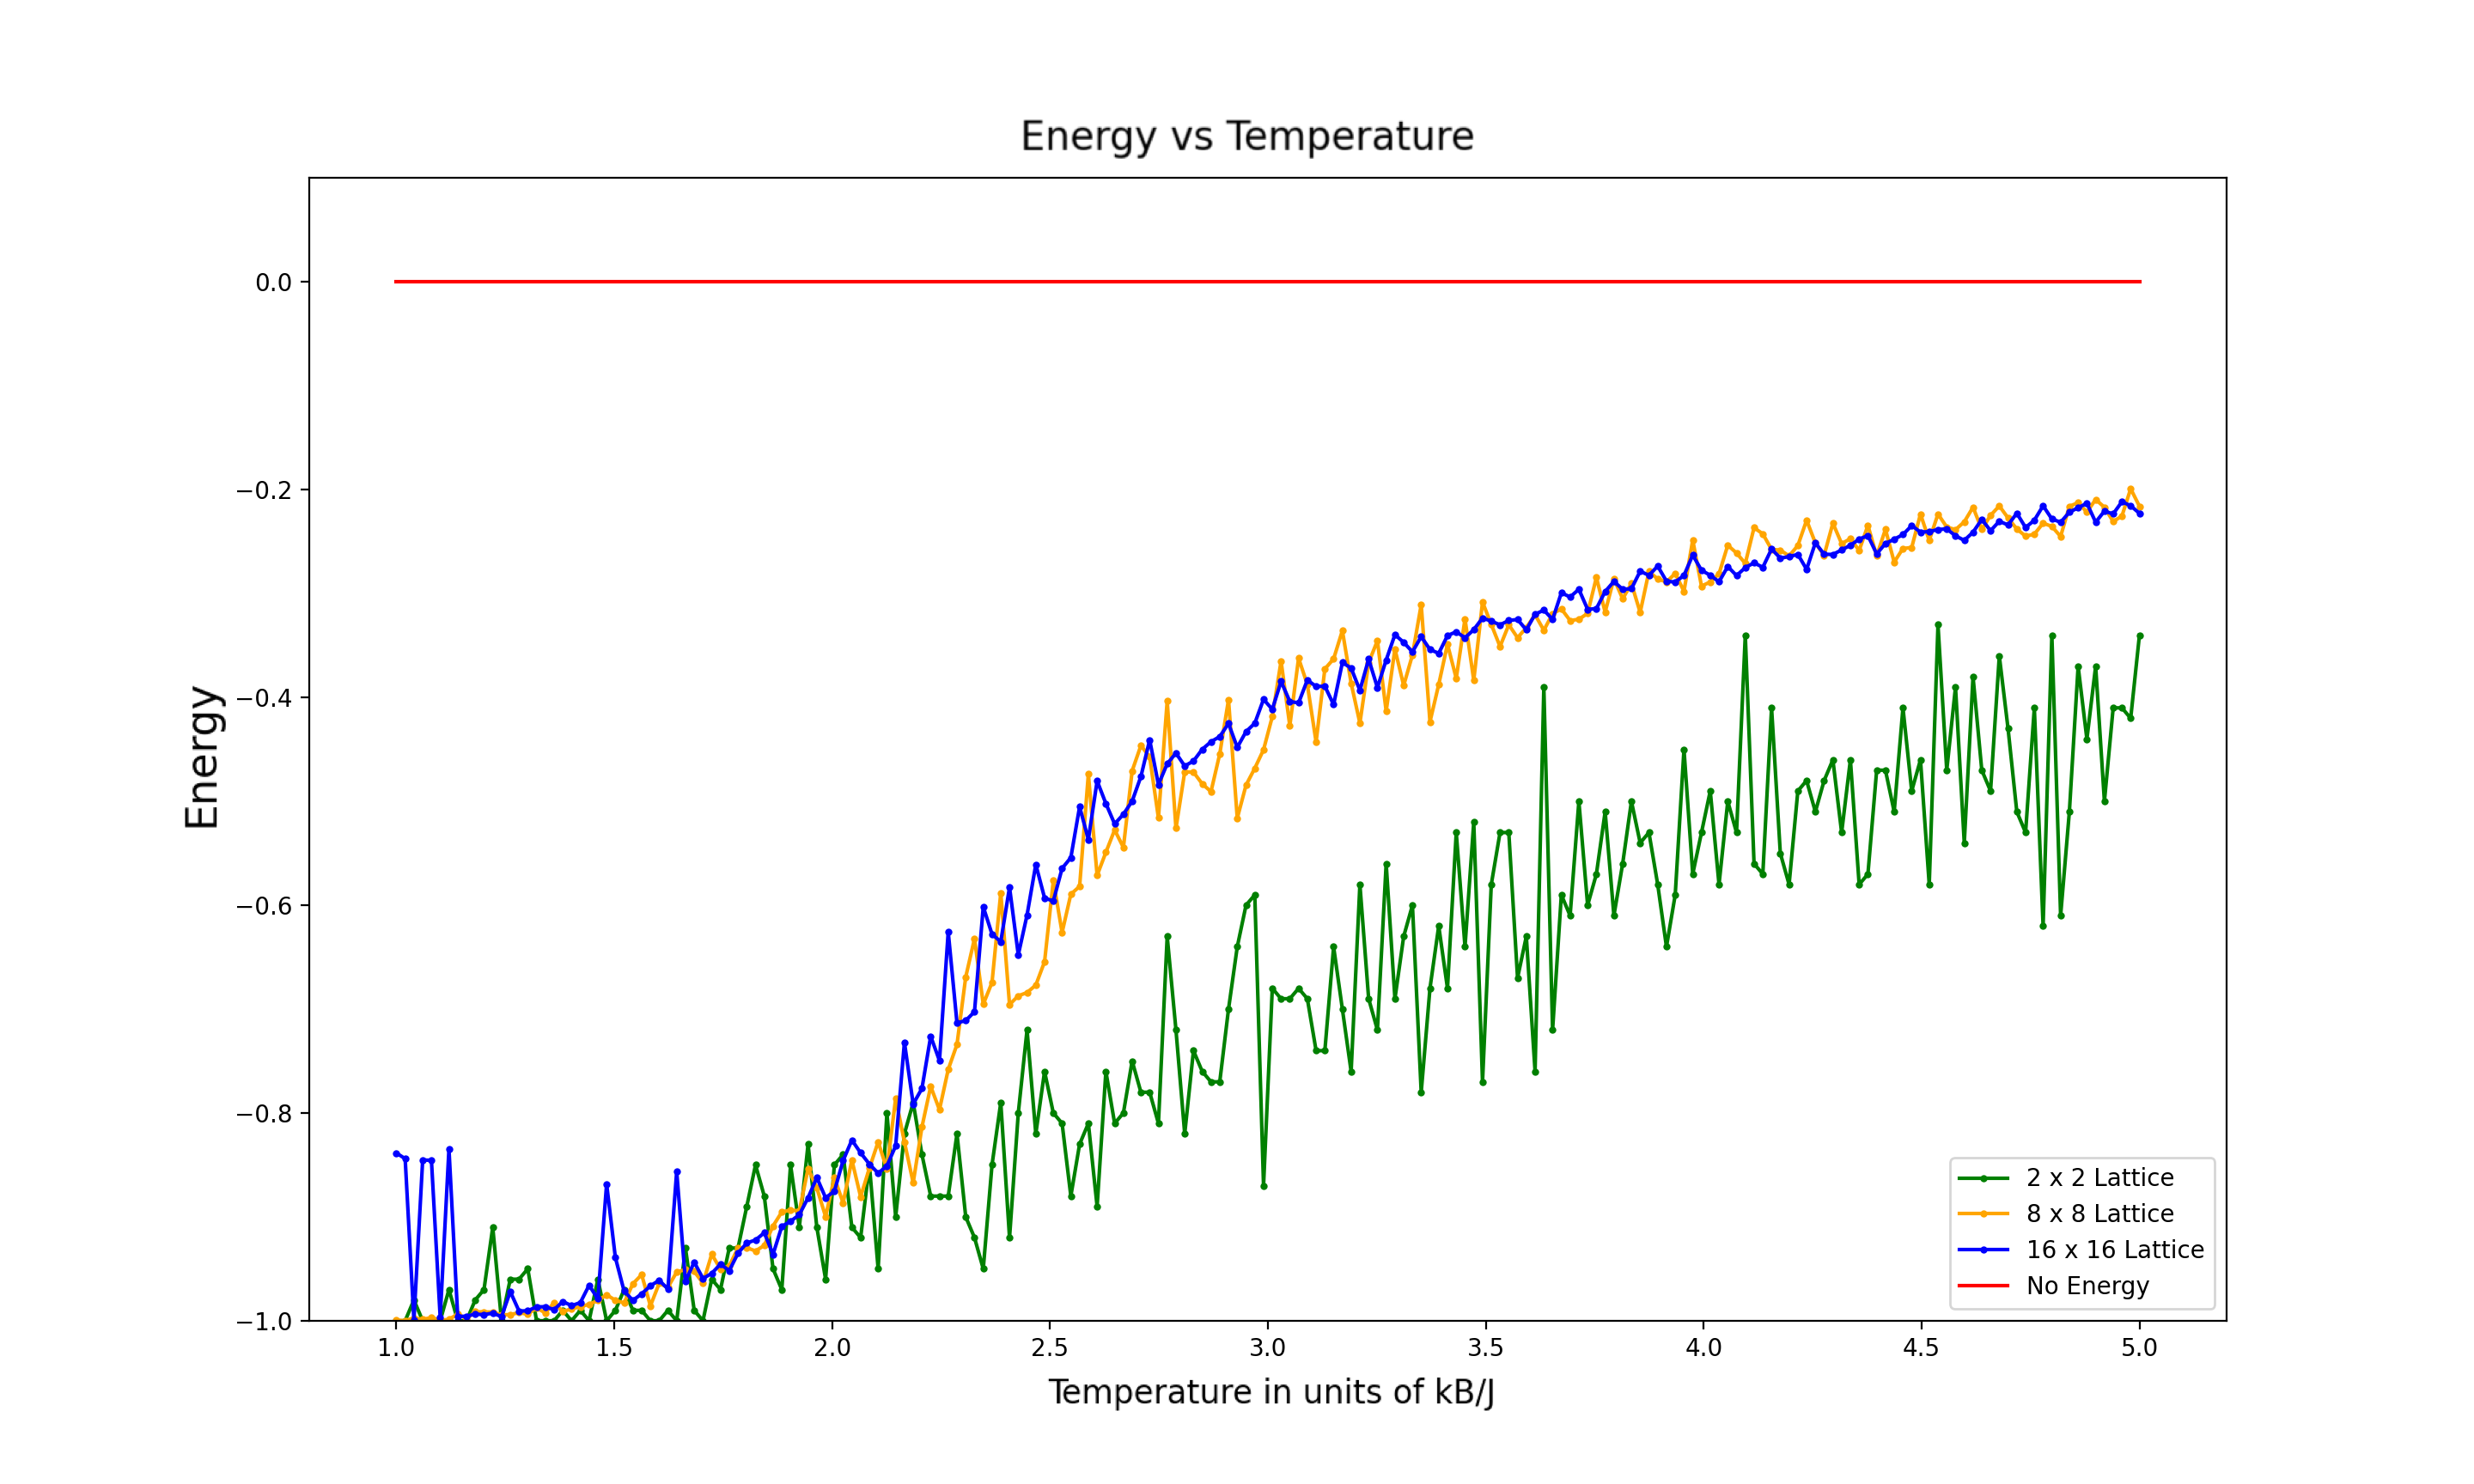
\includegraphics[width=1\linewidth]{energy vs temp.png} 
\caption{Energy vs Temperature}
\label{fig:subim1}
\end{subfigure}
\begin{subfigure}{0.425\textwidth}
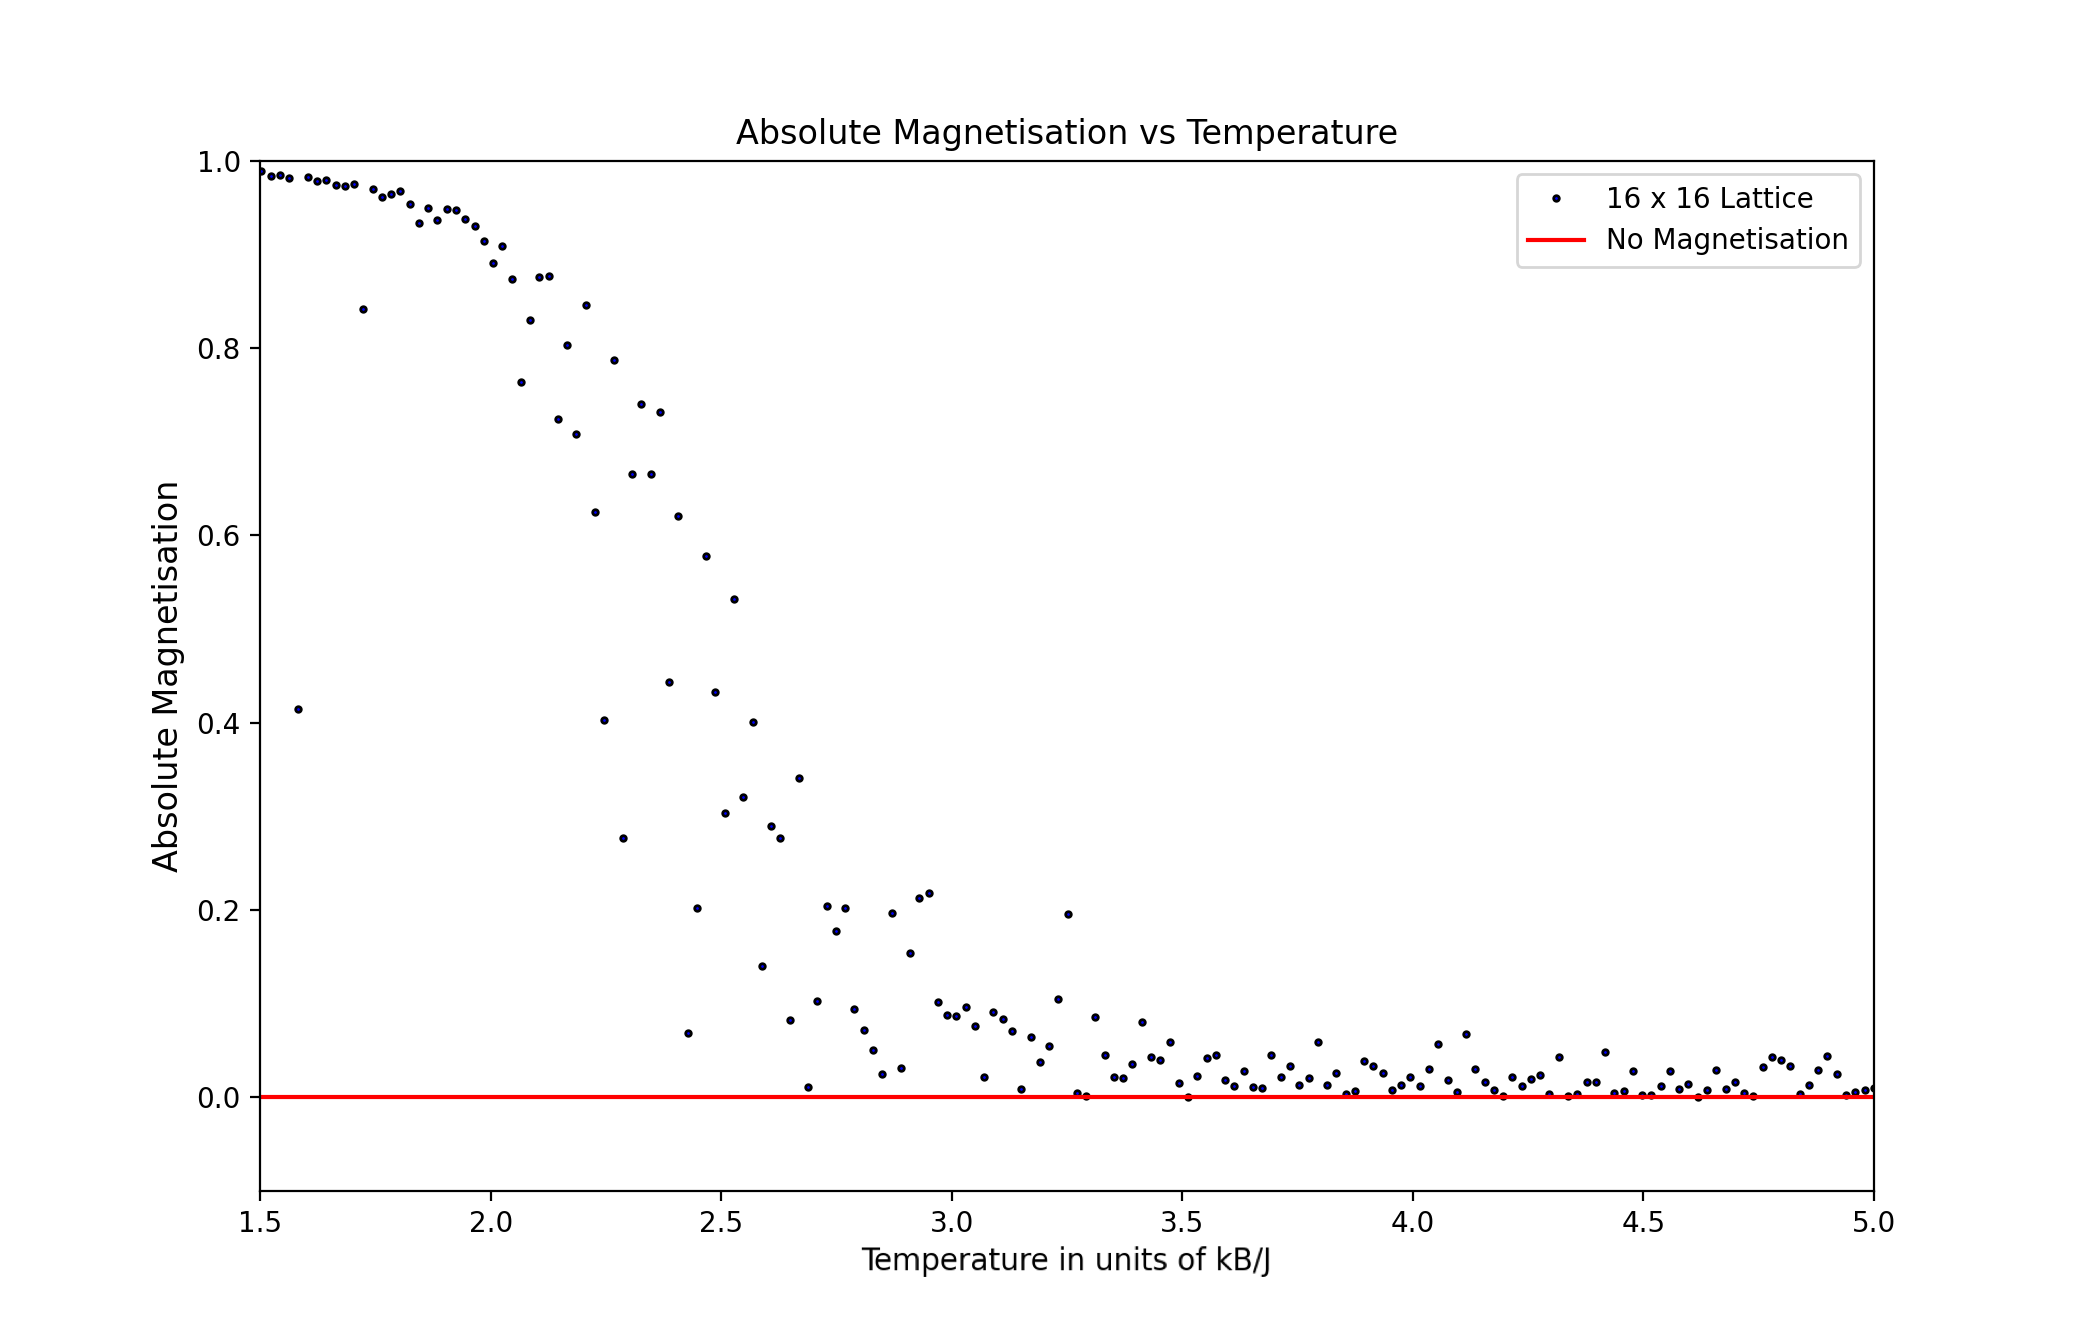
\includegraphics[width=1.1\linewidth,left]{mag vs temp.png}
\caption{Absolute Magnetisation vs Temperature}
\label{fig:subim2}
\end{subfigure}
\caption{Simulations of Energy and Magnetism vs Temperature}
\label{fig:image2}
\end{figure}

Observing Figure 2(a), we notice that as the temperature increases, the net energy decreases but remains negative. This implies that, during lower temperatures, more spins are aligned in the same direction which is a phenomenon we expect due to the Boltzmann distribution. In addition, as temperature is increased, the system of spins becomes increasingly more random which gives rise to the decreasing net energy seen in Figure 2(a).

Along with energy, we can observe magnetisation of the whole system \cite{2}\cite{8}. Treating each spin as a micro-magnet, the mean magnetisation of the system can be defined as,
\begin{align*}
M = \frac{1}{N}\sum_{i}^{N} \sigma_{i} \
\end{align*}
From this it can be deduced that at zero temperature, the magnetisation of the system is 1. It follows that this is the optimal magnetisation of the system and as temperature increases, the magnetisation of the system decreases. This can be depicted in Figure 2(b).

In Figure 2, the energy spikes and the absolute magnetisation drops drastically down to 0. Since the absolute magnetisation of the system drops to 0, this represents a complete loss of magnetism. Thus, the system has undergone a second order phase transition at a critical temperature $T_{c}$. As systems undergo changes over time, sometimes the properties of the system will change abruptly; this is what is known as a $phase$ $transition$. A simple example of a phase transition is a system moving from a solid to a liquid.

As seen in Figure 2(b), the system magnetises at temperatures less than $T_{c}$, this state is called ferromagnetic or ordered. The system is then considered anti-ferromagnetic or disordered for temperatures greater than $T_{c}$. By observing Figure 2, we estimate the critical temperature to be between $2$ and $2.5$. We will provide an analytic result to this critical temperature in the following section.

During a phase transition, we expect the specific heat capacity of the system to increase \cite{8}. We can simulate a specific heat capacity versus temperature plot for a given lattice and observe whether the change in heat capacity occurs at the observed critical temperature.

Using the standard result in equilibrium statistical thermodynamics \cite{7}, heat capacity is defined as,
\begin{align*}
C = \frac{\sigma_{E}^2}{k_{B}T^2}
\end{align*}
where $\sigma_{E}$ denotes the standard deviation of fluctuations in energy and $k_{B}$, $J$, are defined above. We can calculate $\sigma_{E}$ as follows, 
\begin{align*}
\sigma_{E}^2 =  {\langle E^2\rangle} - {\langle E\rangle ^2}
\end{align*}
 where $E$ is defined in equation (3).
 
Now we have an equation for the specific heat capacity, we can plot this against temperature, as seen in Figure 3. 

\begin{figure}[h!]
  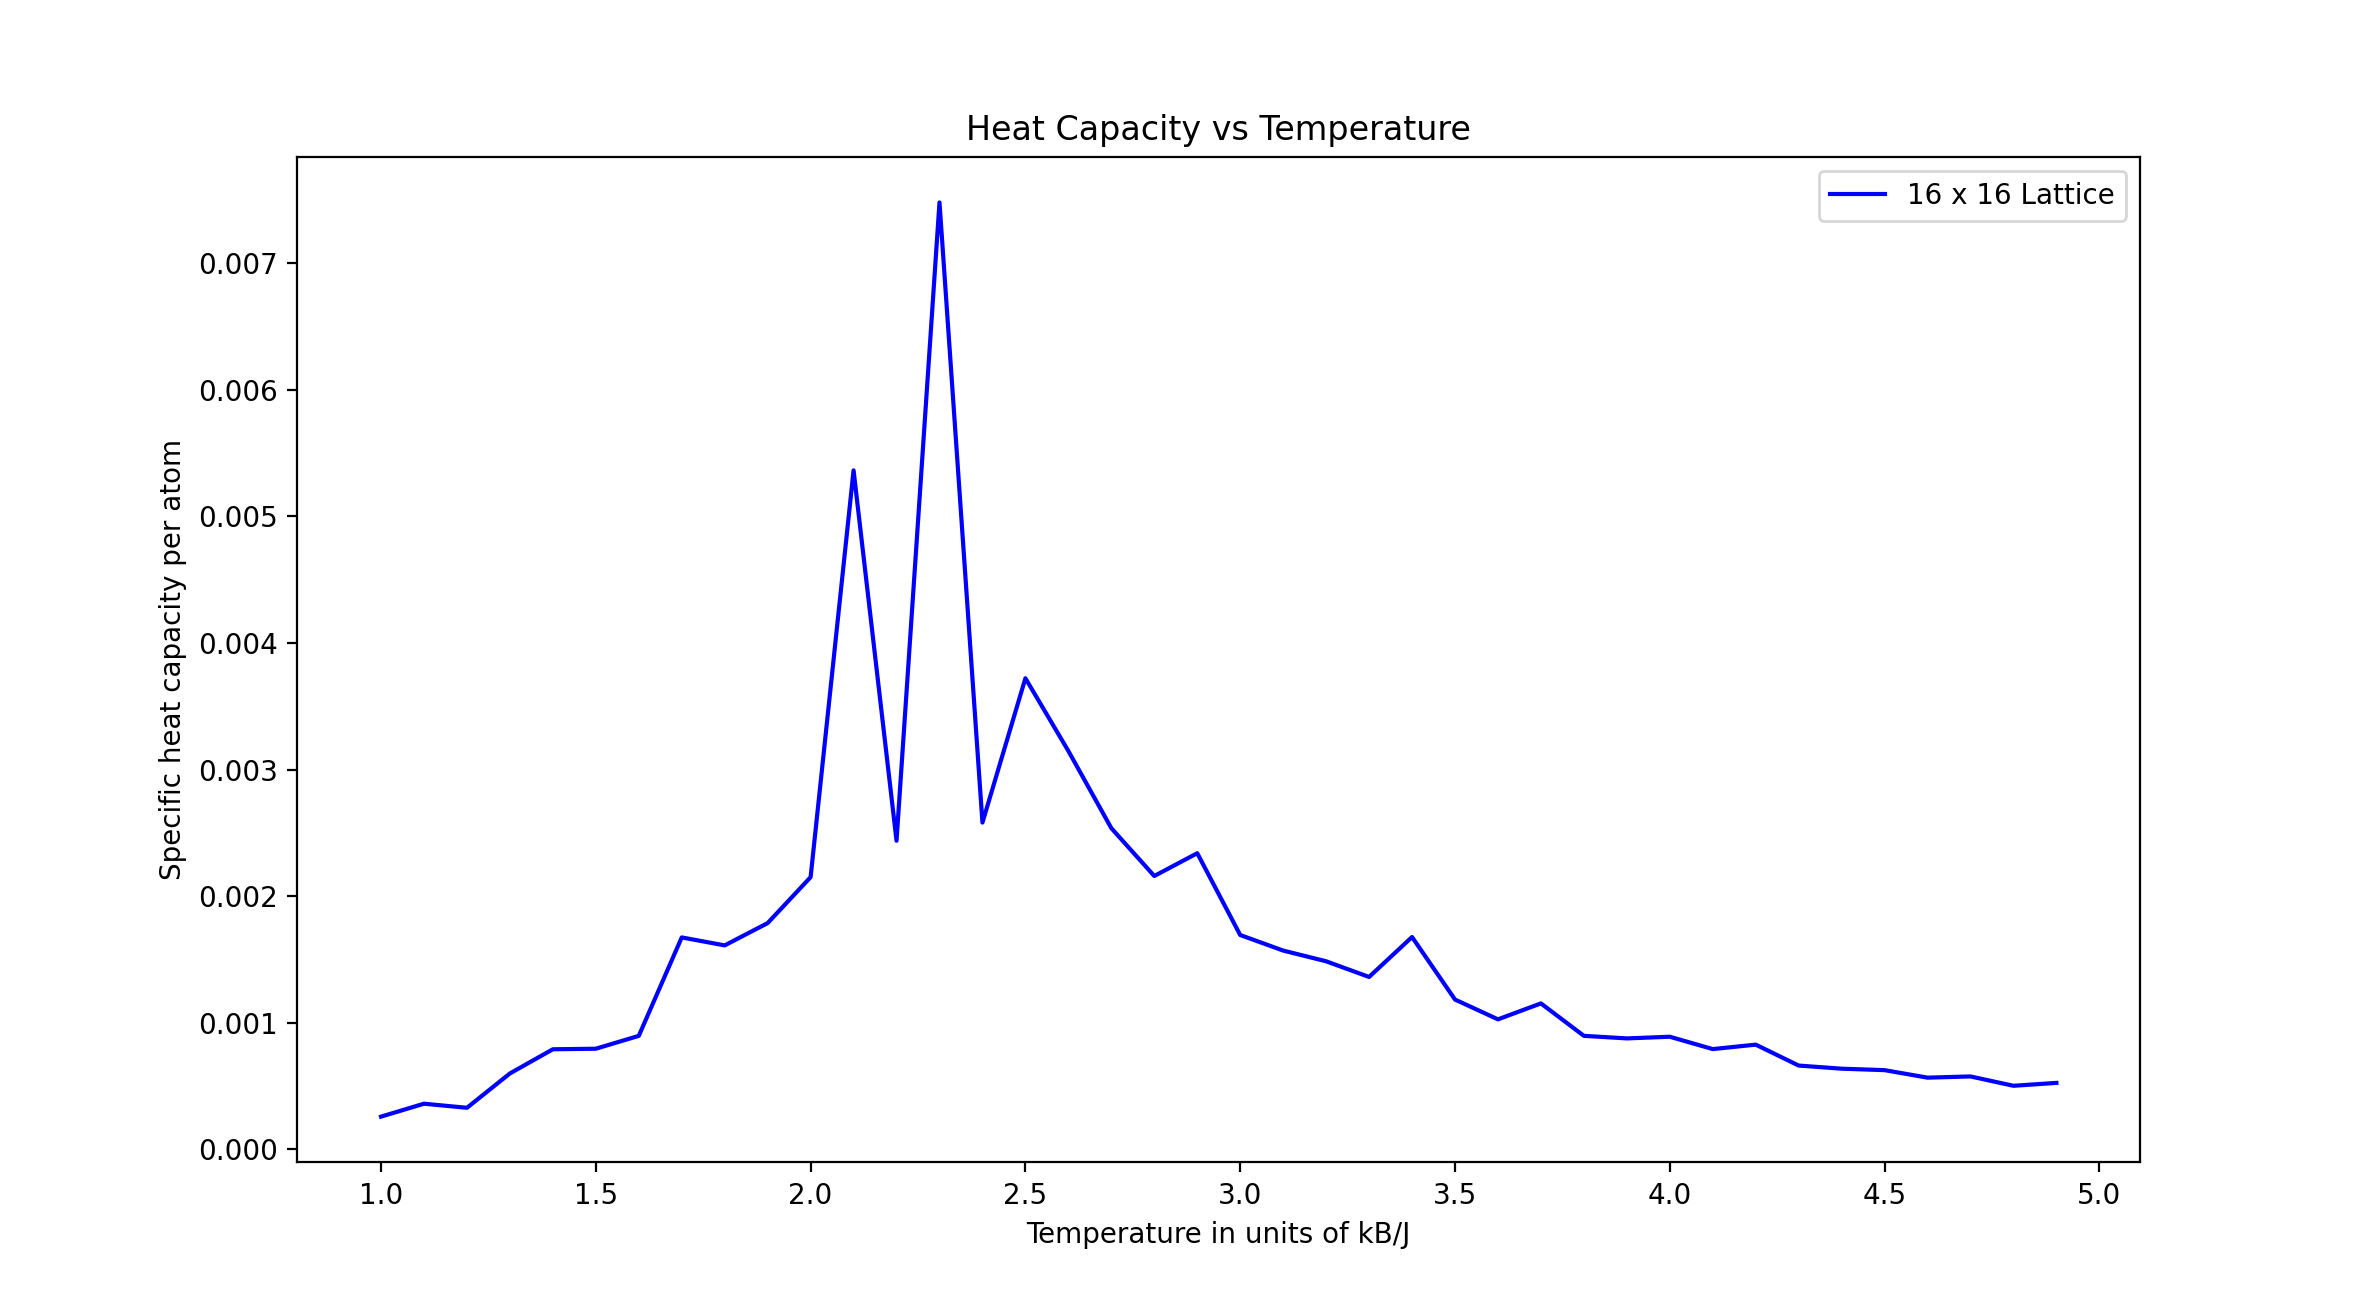
\includegraphics[scale=0.3, center]{heat capacity vs temperature.png}
  \caption{Heat Capacity vs Temperature}
  \label{fig:estimated_mean}
\end{figure} 

It is clear that a large increase or “spike” in the heat capacity occurs between 2 and 2.5. This sharp increase denotes the system going through its phase transition. Thus, we can conclude that the system underwent a phase transition between these temperatures. Although we can observe an estimated critical temperature, we move onto calculating this temperature analytically. With the analytically calculated critical temperature, we can observe the system for temperatures above, equal and below this temperature.

\subsection{Critical Temperature, $T_{c}$, of the 2D Ising Model}

We now adopt an analytical approach for calculating this critical temperature in two dimension. For a one dimension lattice with no external magnetic field, it can be shown that the critical temperature, $T_{c}$, is 0. 

In 1944, Theoretical Physicist, Lars Onsager, obtained the exact, analytical solution of the two-dimensional Ising model \cite{9}. Since this time, there has been no exact solution to the Ising model with an external magnetic field or in higher dimensions. Onsager's solution shows that there exists a second order phase transition at a critical value of,
\begin{align*}
\frac{k_{B}T_{c}}{J} = \frac{2}{\log(1 + \sqrt{2})}
\end{align*}
\cite{8} Generally, with changeable $J$, the critical temperature becomes, 
\begin{align*}
T_{c} = \frac{2J}{\log(1 + \sqrt{2})k_{B}} \approx \frac{2.269185J}{k_{B}}
\end{align*}
As a further simplification, (which is also implemented in our Python simulations), we take $\frac{J}{k_{ B}}$ to be unity. Thus, the critical temperature becomes, 
\begin{align*}
T_{c} = \frac{2}{\log(1 + \sqrt{2})} \approx 2.269185...
\end{align*}
This value of the critical temperature aligns with Figures 2 and 3 where the second order phase transition is clearly illustrated around the critical temperature.

Extending this further, we can observe how the system behaves for temperatures above, equal or below the critical temperature. Recall that we are considering a system with no external magnetic field.

\subsubsection{$T < T_{c}$}

For $T < T_{c}$, the system is in a low temperature phase. Thus, we expect a dominance of one directional spin ($\sigma_{i} \pm 1$) with fluctuations of the opposing directional spin in small clusters or points, as can be seen in Figure 4(a). These small clusters will increase in size as T approaches the temperature at which a second order phase transition begins, $T \rightarrow T_{c}$.

\begin{figure}[h]
\centering
\begin{subfigure}{0.4\textwidth}
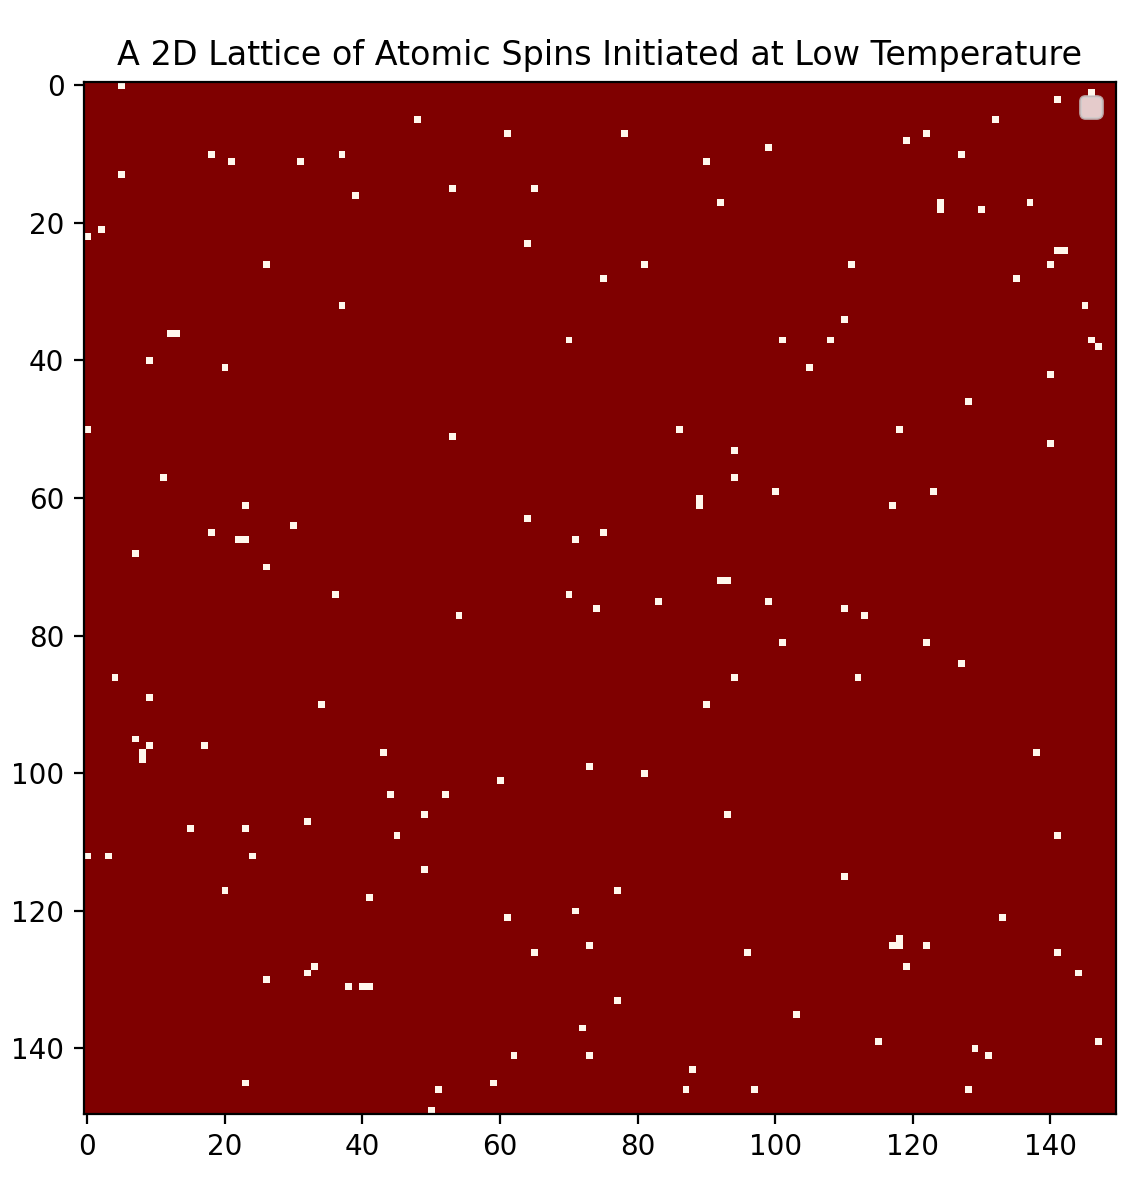
\includegraphics[width=1\linewidth]{2D Low Temperature.png} 
\caption{2D Lattice After 1,000 Metropolis Steps}
\label{fig:subim1}
\end{subfigure}
\begin{subfigure}{0.5\textwidth}
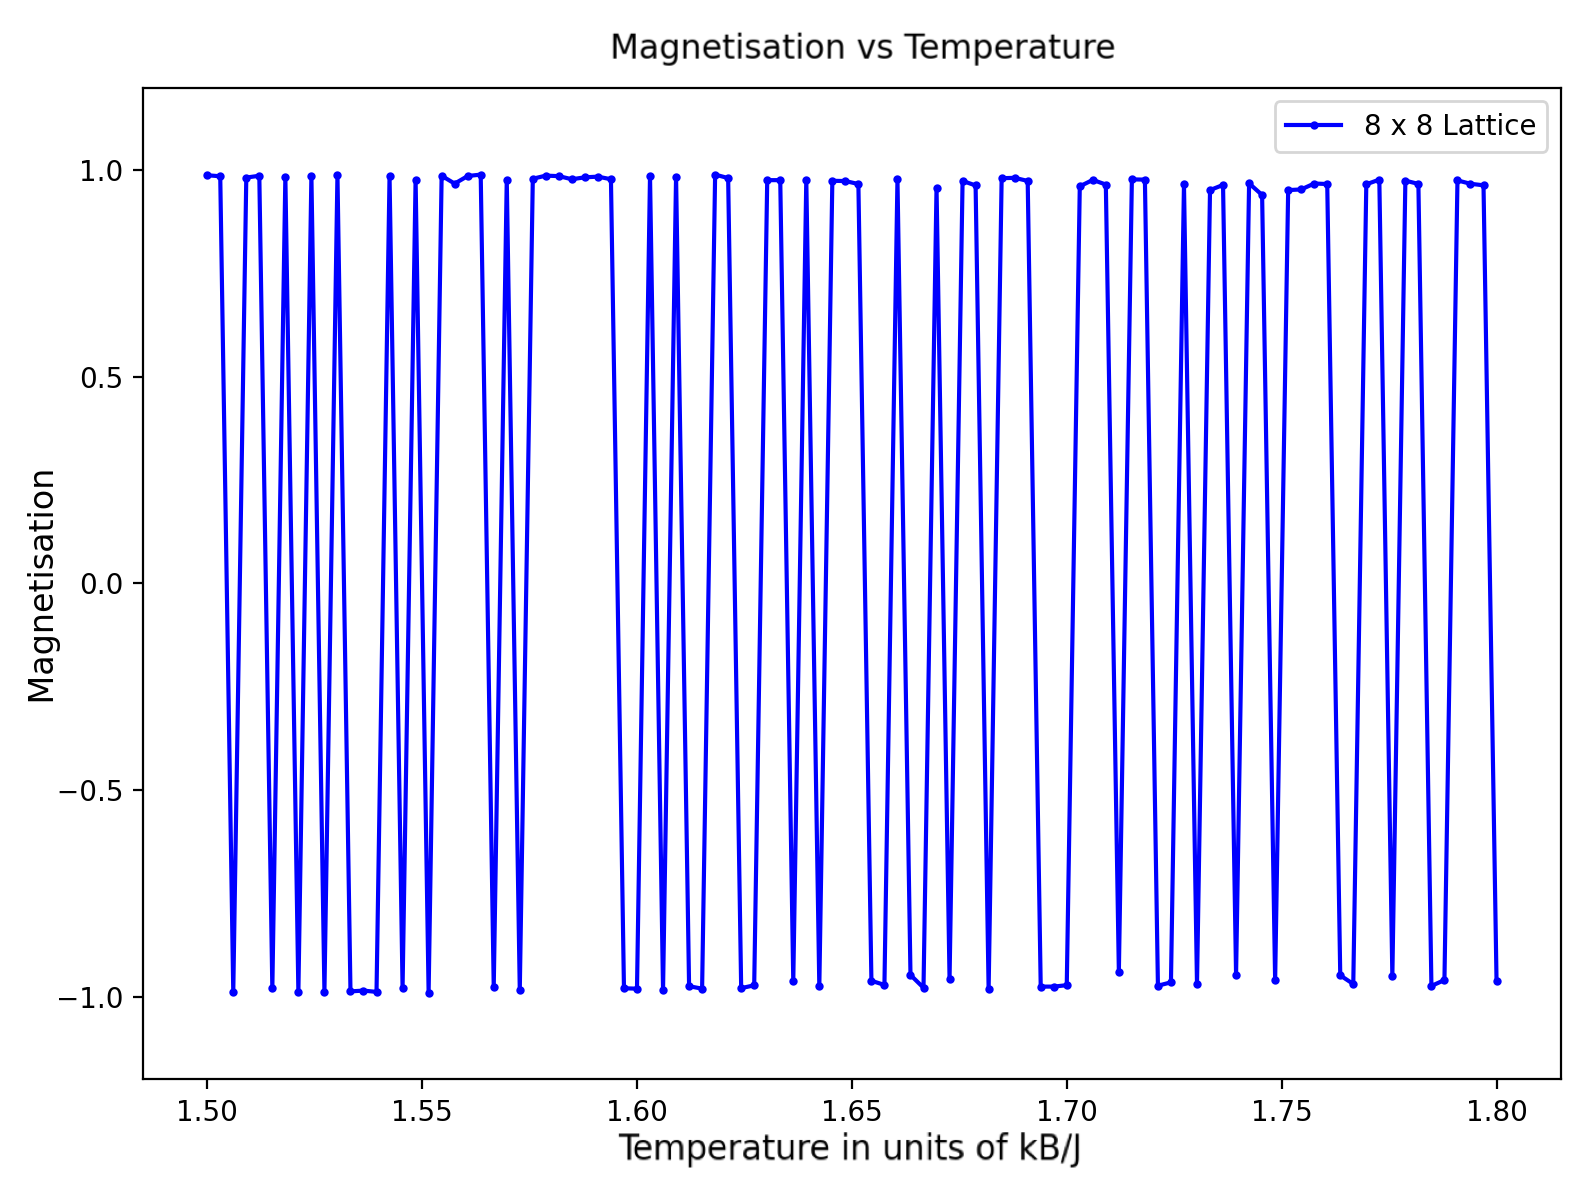
\includegraphics[width=1.1\linewidth,left]{mag vs temp for low temp.png}
\caption{Magnetisation vs Temperature}
\label{fig:subim2}
\end{subfigure}
\caption{2D Ising Model at Low Temperature}
\label{fig:image2}
\end{figure}

Figure 4(b) reiterates that magnetisation is at its optimal during lower temperatures. The figure illustrates that magnetisation only occurs at $\pm{1}$. From this, we can deduce that a system at low temperature will take fewer steps and time to reach equilibrium by the Monte Carlo Metropolis Algorithm.

\subsubsection{$T \approx T_{c}$}

\begin{figure}[h]
\centering
\begin{subfigure}{0.4\textwidth}
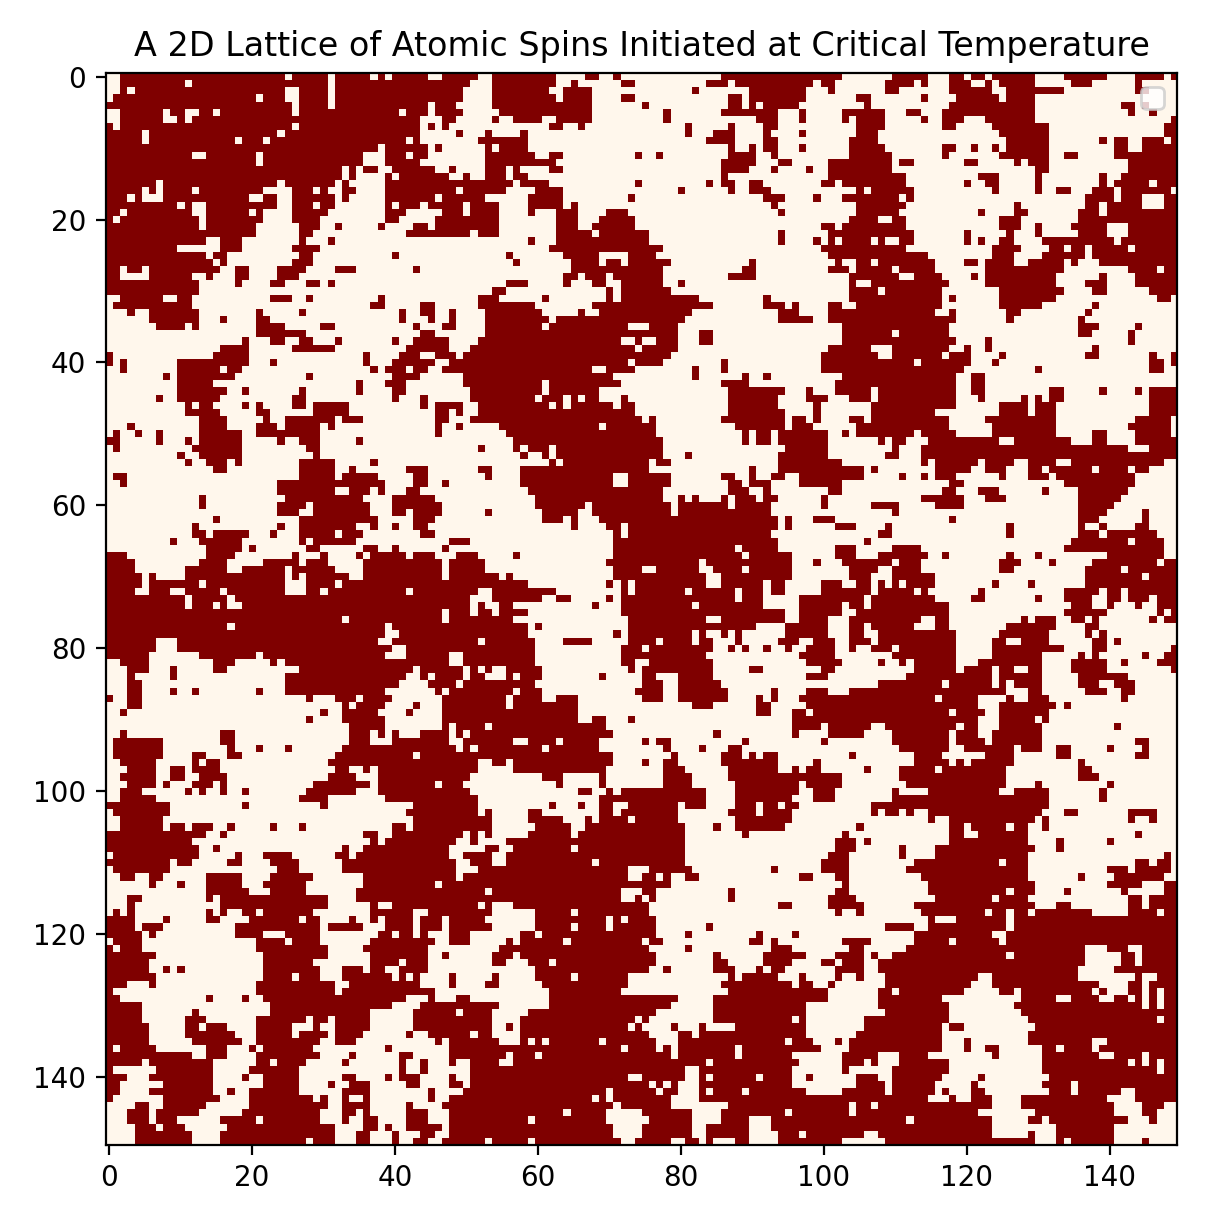
\includegraphics[width=1\linewidth]{2D Lattice Critical Temp.png} 
\caption{2D Lattice After 1,000 Metropolis Steps}
\label{fig:subim1}
\end{subfigure}
\begin{subfigure}{0.5\textwidth}
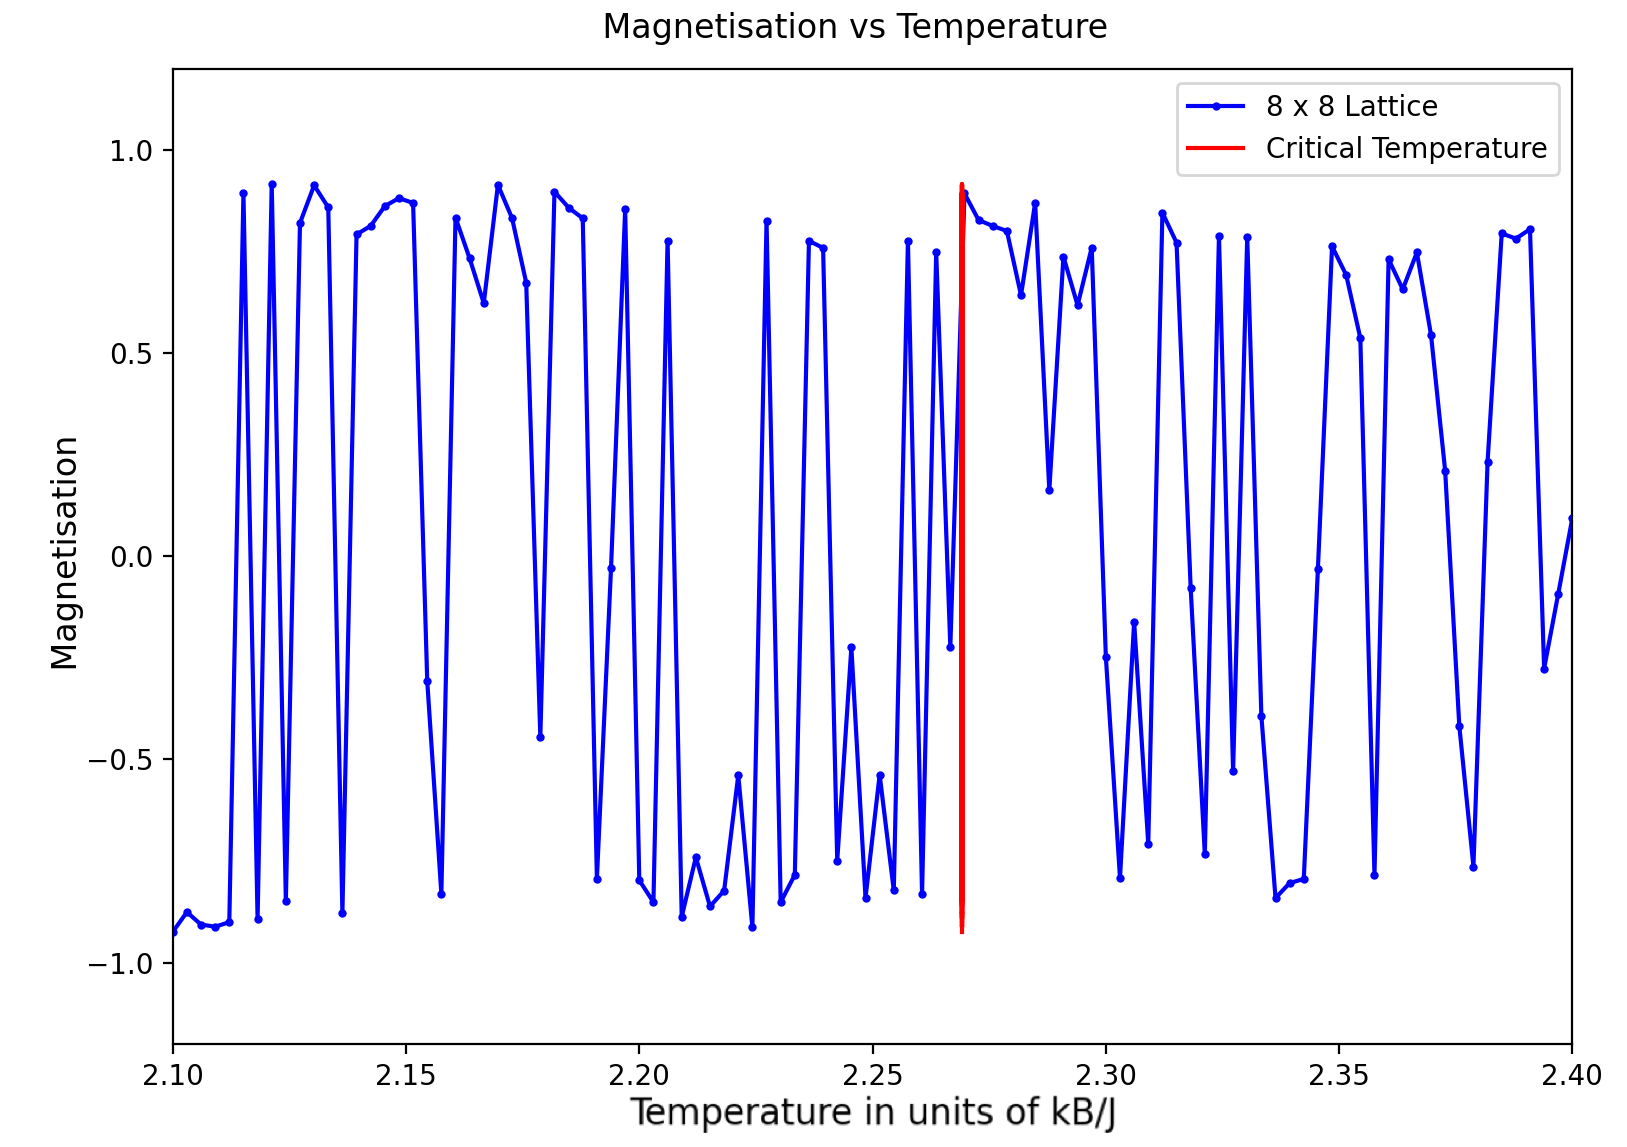
\includegraphics[width=1.1\linewidth,left]{mag vs temp critical temp.png}
\caption{Magnetisation vs Temperature}
\label{fig:subim2}
\end{subfigure}
\caption{2D Ising Model at Critical Temperature}
\label{fig:image2}
\end{figure}

At critical temperature, we expect to observe the system undergoing the second order phase transition, as predicted by Onsager's solution. During this phase transition, fluctuations in the spins will occur with no clear dominance of one spin, as depicted in Figure 5(a). Similarly, the magnetisation of the system is expected to fluctuate as a result of the fluctuations in spins. This is illustrated in Figure 5(b) where the magnetisation of the system differs around the critical temperature. 

A system with temperature at its critical temperature will result in signs of decay in the alignment as the system passes through iterations of the Metropolis Algorithm. The system can reach equilibrium but due to the declining magnetism, the system cannot maintain equilibrium.

\subsubsection{$T > T_{c}$}

At high temperatures, we know that the system's energy will increase and thus, create an imbalance between the alignment of spins. This has already been depicted in Figure 2. Owing to this, we expect the system to appear random with no dominance of one spin and no obvious patterns; the system will appear completely random. This observation can be shown in Figure 6(a). 

Similarly, the overall magnetisation of the system fluctuates around 0 which suggests that the system is anti-ferromagnetic; it has little or no influence by magnetism. This is reiterated through the lack of aligned spins in Figure 6(a). 

\begin{figure}[h]
\centering
\begin{subfigure}{0.37\textwidth}
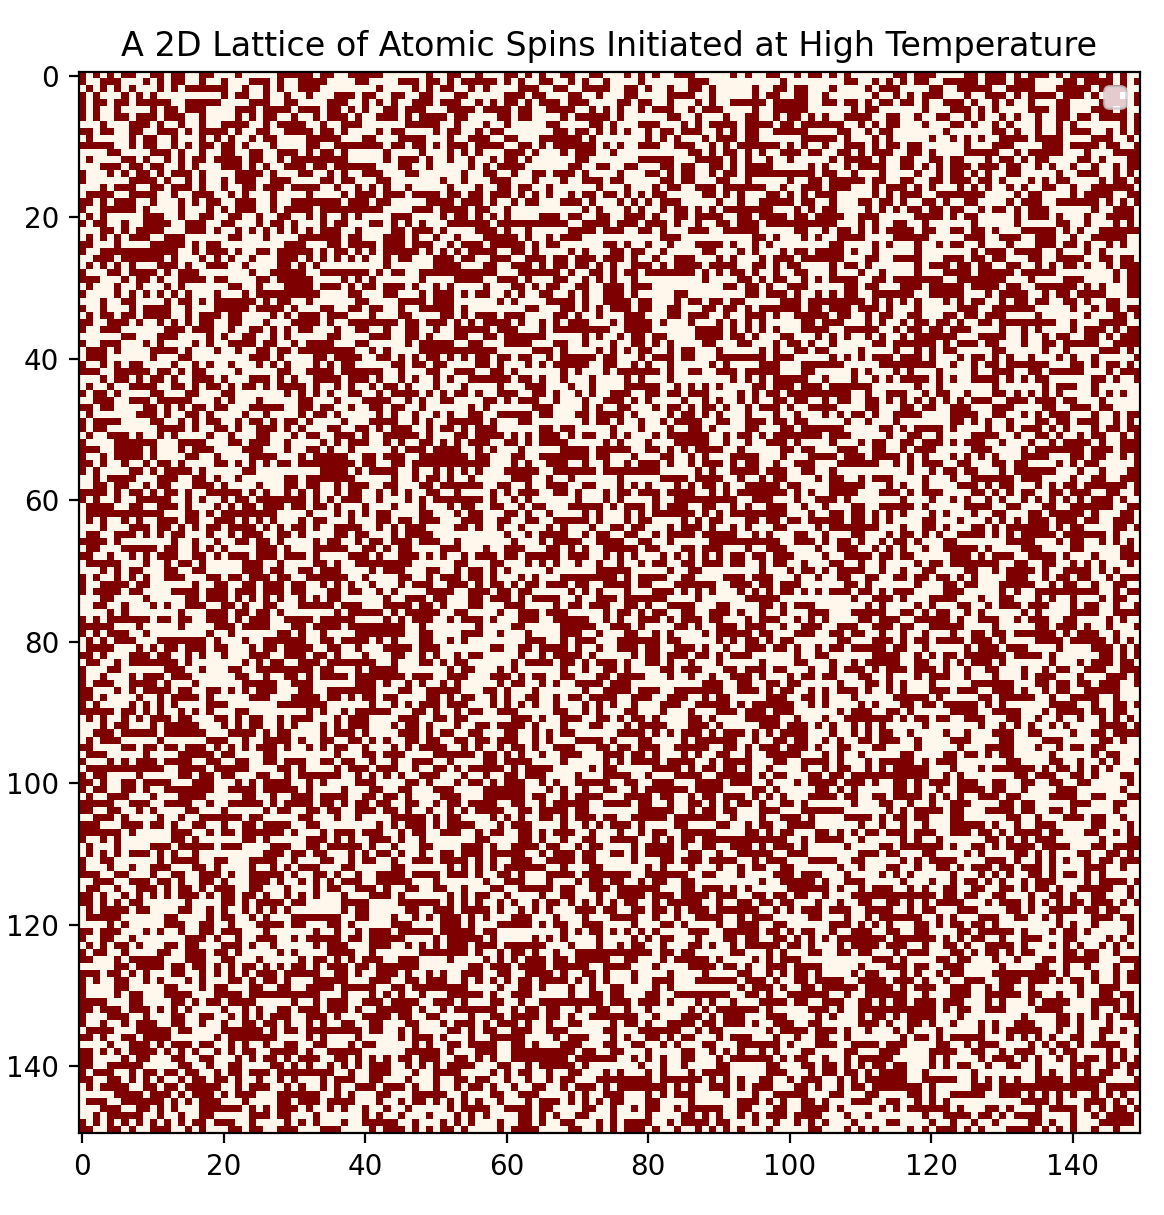
\includegraphics[width=1\linewidth]{2D Lattice High Temperature.png} 
\caption{2D Lattice After 1,000 Metropolis Steps}
\label{fig:subim1}
\end{subfigure}
\begin{subfigure}{0.5\textwidth}
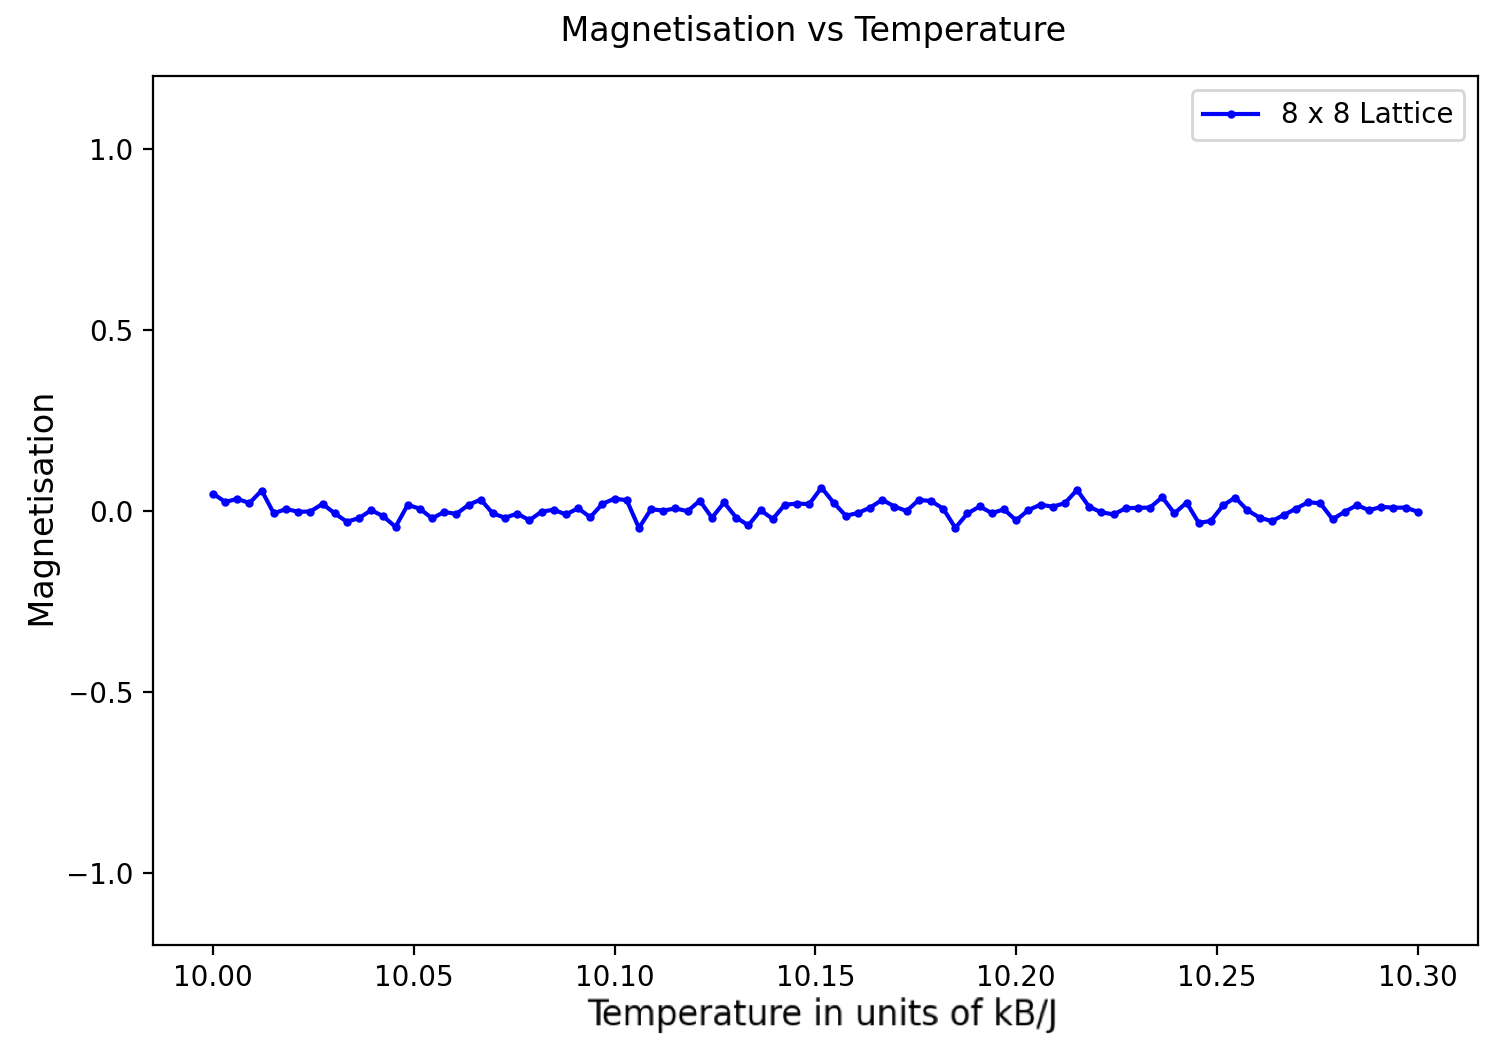
\includegraphics[width=1.02\linewidth,left]{mag vs temp high temp.png}
\caption{Magnetisation vs Temperature}
\label{fig:subim2}
\end{subfigure}
\caption{2D Ising Model at High Temperature}
\label{fig:image2}
\end{figure}

As a result of the high temperature, over time the system will be unable to reach equilibrium, regardless of how many Monte Carlo Metropolis simulations are run. When considering the Metropolis approach to simulating the Ising model, fixed temperatures below the critical temperature are often considered. Commonly, simulations are run with $\beta$ = $\frac{1}{k_{B}T} \approx 0.4$.

\subsection{Simulating the 2D Ising Model Over Time}

We consider the 2D Ising model with energy defined in (3) with $\beta = 0.4$ and, exchange energy, $J$, and Boltzmann constant, $k_{B}$, to be unity. We will begin the system in an anti-ferromagnetic (disordered) state and observe the system as it iterates through the Metropolis Algorithm (3.1).

We observe six simulations of the system as it transitions through various Monte Carlo Metropolis iterations (steps) as can be seen between Figures 7 to 12.

\begin{figure}[!htb]
\minipage{0.32\textwidth}
  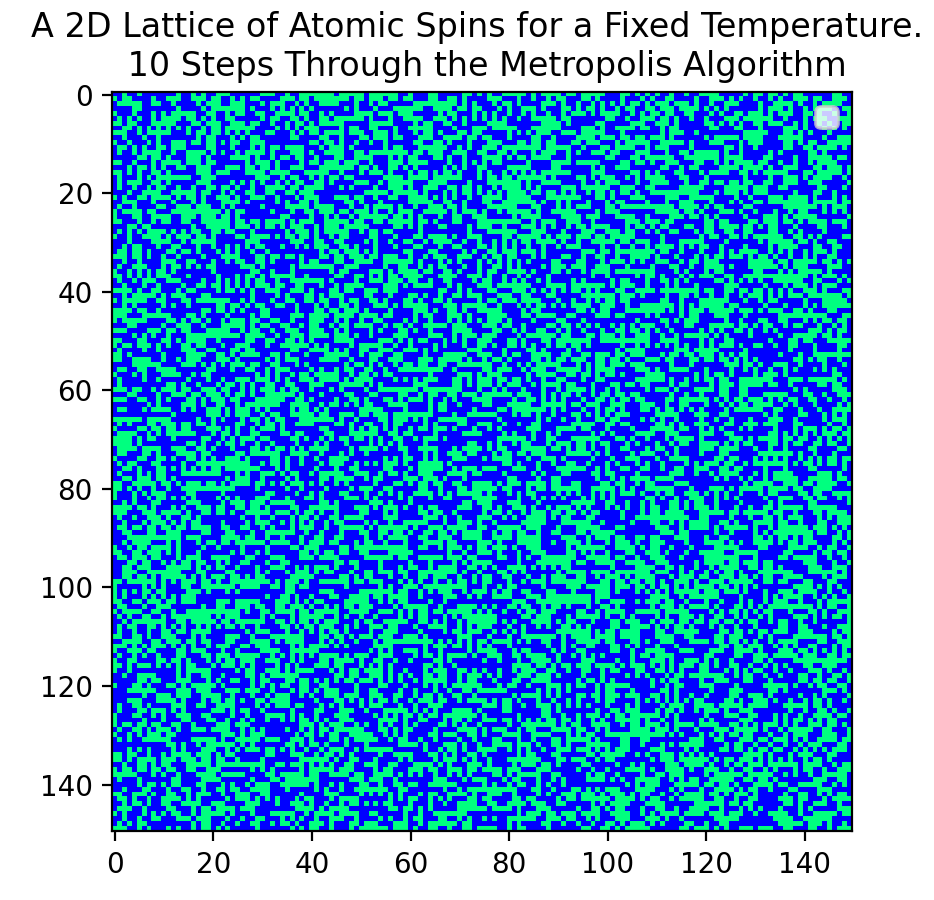
\includegraphics[width=\linewidth]{10 steps.png}
  \caption{10 Steps}\label{fig:10steps}
\endminipage\hfill
\minipage{0.32\textwidth}
  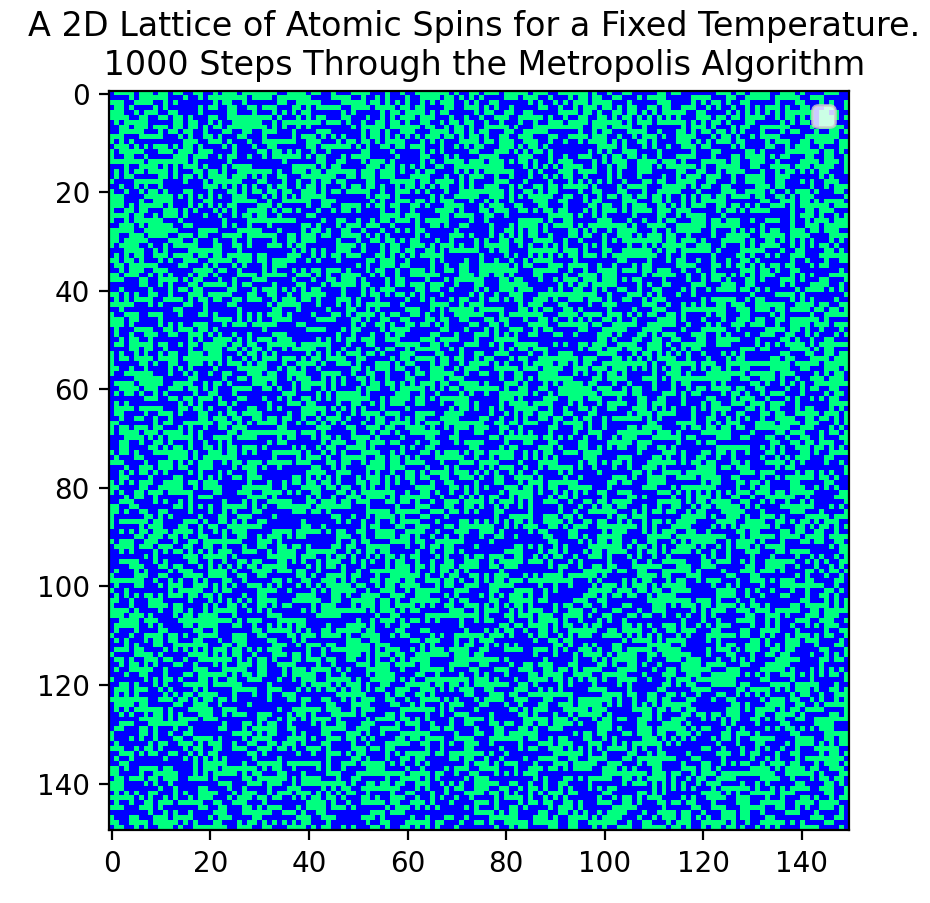
\includegraphics[width=\linewidth]{1000 steps.png}
  \caption{1,000 Steps}\label{fig:100steps}
\endminipage\hfill
\minipage{0.32\textwidth}%
  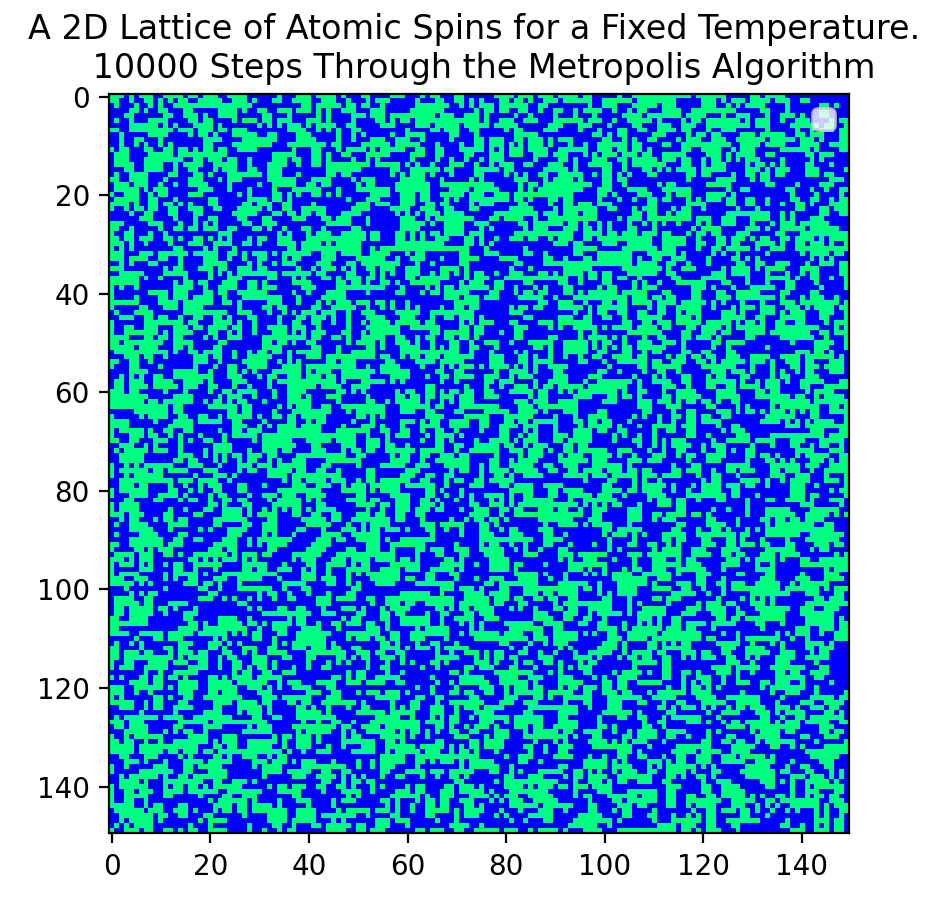
\includegraphics[width=\linewidth]{10,000 steps.png}
  \caption{10,000 Steps}\label{fig:1000steps}
\endminipage
\end{figure}

\begin{figure}[!htb]
\minipage{0.32\textwidth}
  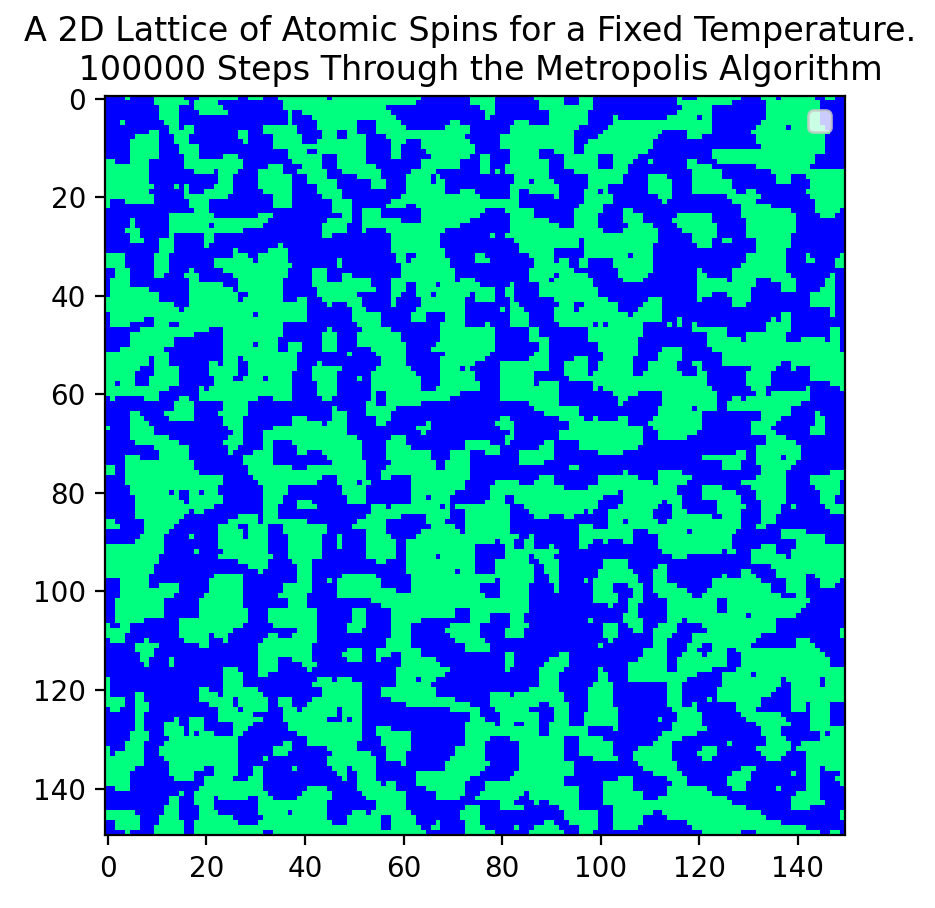
\includegraphics[width=\linewidth]{100,000 steps.png}
  \caption{100,000 Steps}\label{fig:10steps}
\endminipage\hfill
\minipage{0.32\textwidth}
  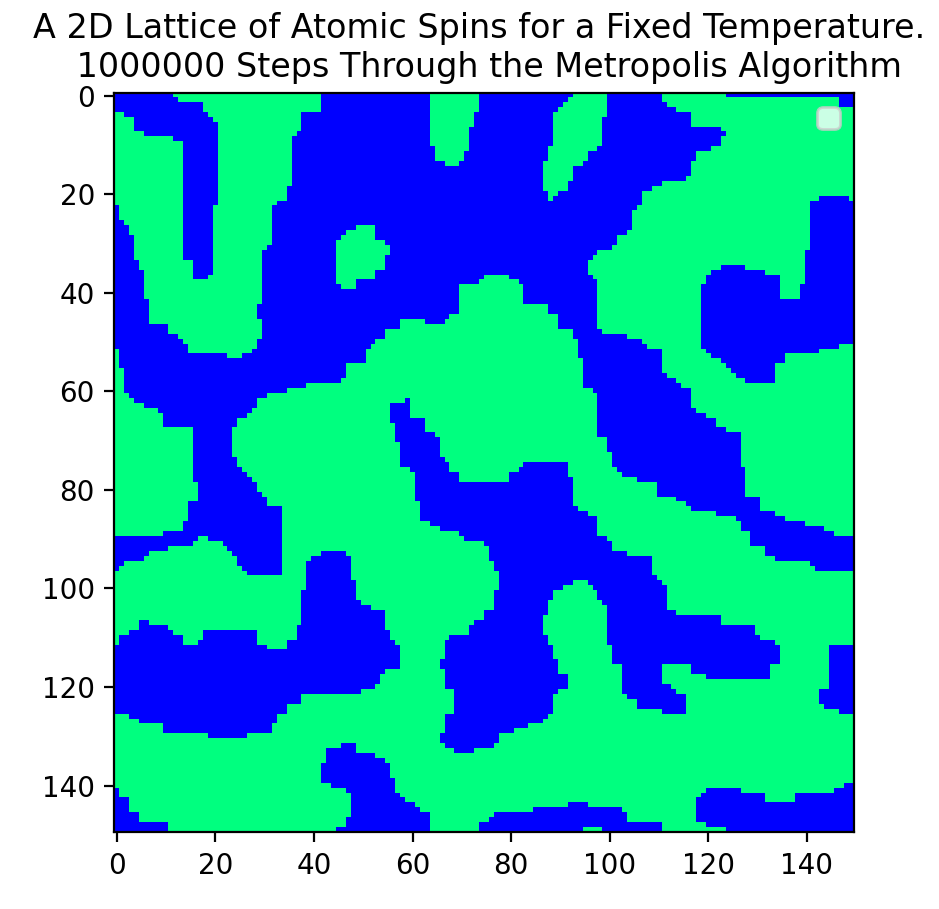
\includegraphics[width=\linewidth]{1,000,000 steps.png}
  \caption{1,000,000 Steps}\label{fig:100steps}
\endminipage\hfill
\minipage{0.32\textwidth}%
  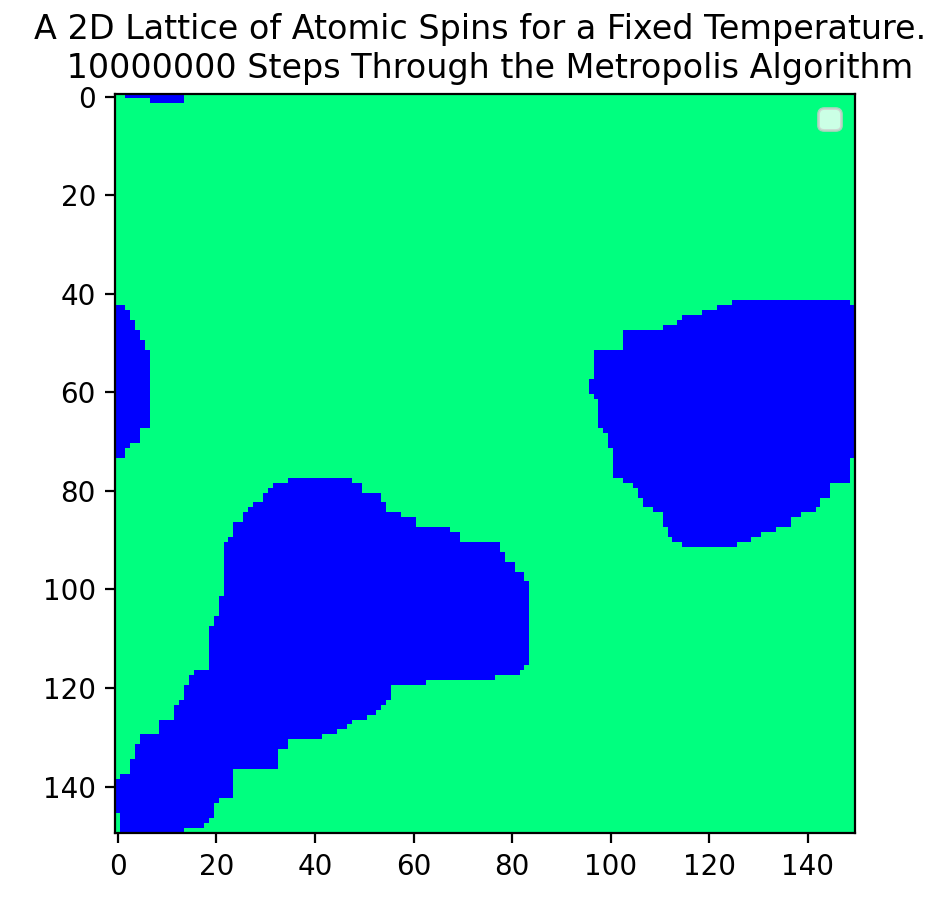
\includegraphics[width=\linewidth]{10,000,000 steps.png}
  \caption{10,000,000 Steps}\label{fig:1000steps}
\endminipage
\end{figure}

For a fixed temperature lower than the critical temperature, the disordered system tends towards an ordered, ferromagnetic system as it passes through increased steps of the Metropolis algorithm. This phenomenon reiterates the power behind Monte Carlo methods, specifically the Metropolis algorithm; we are able to take a two-dimensional anti-ferromagnetic (disordered) system and influence a phase transition that turns the system ferromagnetic (ordered). 

The two dimensional Ising model is fundamental as it allows the identification of phase transitions and through Monte Carlo methods, gauges approximate methods of solutions that can then be tested against the analytic solution.

\section{Conclusion}
We have seen that Monte Carlo methods can be used to influence a state of order to a system. Particularly, incorporating the Boltzmann distribution, Metropolis algorithm and Ising model to successfully reproduce the qualitative behaviour of specific types of magnetic material. 

Monte Carlo methods are fundamental to mathematics and physics and give accurate solutions to problems using random numbers. Further applications and studies may include exploring the Ising model under the influence of an external magnetic field, the 3D Ising model or other models including Potts and Heisenburg. 

% \section{References}
\begin{thebibliography}{5}
\bibitem{1}\href{https://arxiv.org/pdf/hep-ph/0006269.pdf}{Weinzierl, S. “Introduction to Monte Carlo Methods”. Nikhef's Theoretical Physics Group. 2000.}
\bibitem{2} Harlen, O.G and Evans, R.M.L. “Using Random Numbers to Solve Problems in Mathematics and Physics”. MATH3001 Project in Mathematics. 2020/21.
\bibitem{3} \href{https://reader.elsevier.com/reader/sd/pii/S1007570409003517?token=5C265B5A35134BF073C921936D14B965297B5F00FF3AD6194363AD5D2764B57E4814ED5B647AAE9FBBC7C44F5601547E}{Kastner, M. “Monte Carlo Methods in Statistical Physics: Mathematical Foundations and Strategies”. Elsevier. 2009, pp.1589–1602.}
\bibitem{4} Kalos, M.H. and Whitlock, P.A . “Monte Carlo Methods”. 2nd Edition. USA. Wiley - VCH, 2008.
\bibitem{5}\href{https://bayes.wustl.edu/Manual/EquationOfState.pdf}{Metropolis, N., Rosenbluth, A.W., Rosenbluth, M.N. and Teller, A.H. “Equation of State Calculations by Fast Computing Machines”. Journal of Chemical Physics. 1953, Volume 21, pp.1087-1092}
\bibitem{6}\href{https://arxiv.org/pdf/0808.2902.pdf}{Robert, C. and Casella, G. “A Short History of Markov Chain Monte Carlo”. Institute of Mathematical Statistics. 2011, Volume 26, pp.102-115}
\bibitem{7}\href{http://farside.ph.utexas.edu/teaching/329/lectures}{Fitzpatrick, R. “The Ising Model”. PHY329 Computational Physics. 2014.}
\bibitem{8} \href{https://arxiv.org/pdf/0803.0217.pdf}{Kotze, J. “Introduction to Monte Carlo Methods for an Ising Model of a Ferromagnet”.}
\bibitem{9} \href{https://link.springer.com/article/10.1007/BF02980577}{Ising, E. Beitrag zur Theorie des Ferromagnetismus. Z. Physik 31, 253–258, 1925.}
\end{thebibliography}





\end{document}



